% Building upon the algorithmic foundations summarized in Section~III, this section focuses on the design phase of PECs, where DRL enables data-driven optimization and design automation. To contextualize the role of DRL, the following discussion outlines the fundamental challenges of converter design. 

% Design in PECs, encompassing topology selection, parameter tuning, and reliability assurance, often involves high-dimensional and nonlinear optimization problems subject to stringent performance, thermal, and manufacturability constraints. Traditional design workflows, which rely heavily on expert heuristics, manual iterations, and time-consuming simulations, typically result in slow convergence and extended development cycles. To address these challenges, recent advances in DRL introduce a data-driven paradigm capable of autonomously learning design strategies through direct interaction with the environment. 
% Unlike traditional heuristic optimization approaches, DRL adaptively explores complex, high-dimensional design spaces while efficiently handling sparse rewards and conflicting objectives. Owing to this adaptability, DRL has shown strong potential for optimizing three major design tasks: topology exploration, parameter optimization, and multiobjective trade-off analysis.
% Fig.~\ref{fig:topo_overview} illustrates the systematic workflow of DRL-assisted converter design.

% %%%%%%%%%%%%%%%%%%%%%%%%%%%%%%%%%%%%%%%%%%%%%%%%%%%
% \subsection{Topology Exploration}
% \label{sec:topo_explore}
% %%%%%%%%%%%%%%%%%%%%%%%%%%%%%%%%%%%%%%%%%%%%%%%%%%%

% Topology exploration in PECs has recently advanced through the integration of artificial intelligence, particularly RL and graph-based generative modeling. Existing approaches can be broadly categorized into three classes: adjacency-matrix-driven strategies, graph-learning frameworks, and hybrid generative models.

% Adjacency-matrix-driven methods, such as the Q-learning framework proposed by Chen et al.~\cite{9615058}, encode circuit connections as custom adjacency matrices and iteratively construct converter topologies. The RL agent progressively adds components under reward functions enforcing electrical feasibility, loop integrity, and voltage-second balance, thereby achieving fully automatic topology deduction without expert intervention. 


% \begin{figure}[!t]
%     \centering
%     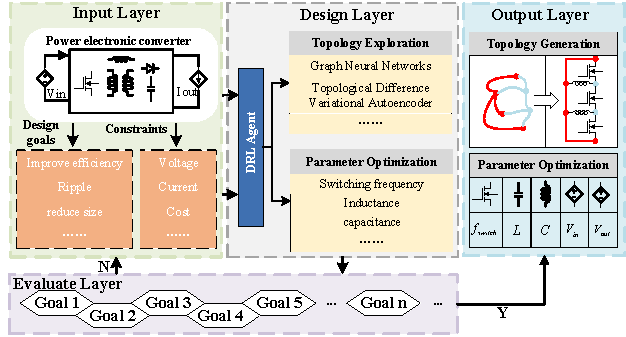
\includegraphics[width=\linewidth]{fig/design_overview.pdf}
%     \caption{Flowchart of DRL-assisted design for PECs.}
%     \label{fig:topo_overview}
% \end{figure}

% Building upon this foundation, graph-based deep learning approaches~\cite{liang2022learning,10012061} represent circuits as undirected graphs processed by graph neural networks (GNNs) coupled with actor-critic algorithms such as PPO. Liang \textit{et al.}~\cite{liang2022learning} employed a GNN-driven PPO agent to sequentially attach functional blocks, reducing search complexity from exponential to near-linear and cutting switch count by more than 30\% relative to combinatorial baselines. Dong \textit{et al.}~\cite{10012061} extended this framework by embedding constraint management into a PPO-GNN architecture, ensuring compliance with voltage and current stress limits. Their method reduced generation time for complex eight-port topologies by an order of magnitude while lowering voltage and current stresses by 50\% and 31\%, respectively.  

% Complementing these graph-based strategies, Fan \textit{et al.}~\cite{fan2021specification} proposed an upper-confidence-bound-tree (UCT)-based RL framework that automates converter design directly from target specifications. The agent explores the topology space using specification-encoded reward signals, guided by a default policy capable of exploiting small offline datasets to accelerate learning. This hybrid strategy generated energy-efficient converter topologies for diverse voltage-conversion ratios, achieving up to 67\% faster topology generation than prior optimization schemes while discovering novel, non-intuitive configurations.

% More recently, hybrid generative frameworks have emerged that integrate variational autoencoders (VAEs) with RL to enhance diversity and controllability. Xu \textit{et al.}~\cite{xu2022power} developed the TopoDiffVAE, a topological-difference VAE coupled with RL, where the decoder serves as a topology generator guided by constraint-aware rewards preventing short circuits and enforcing component limitations. This hybrid paradigm accelerates topology generation and improves structural validity compared with purely data-driven models.

% Collectively, these advances demonstrate that the synergy of RL, GNNs, UCT-based search, and deep generative modeling provides a scalable, automated pathway for converter topology discovery. 
% The integration of domain-specific reward shaping and constraint management ensures physical feasibility, while the modular nature of these frameworks enables adaptation to diverse architectures and operating conditions. 
% Table~\ref{tab:Topology_Exploration} summarizes representative DRL algorithms for topology exploration in PECs.

% \begin{table*}[t]
% \centering
% \caption{Summary of Topology Exploration in Power Electronic Converters Using DRL}
% \label{tab:Topology_Exploration}
% \renewcommand{\arraystretch}{1.25}
% \resizebox{\textwidth}{!}{
% \begin{tabular}{@{}l l p{3.4cm} l p{5.6cm}@{}}
% \toprule
% \textbf{Topology Type} & \textbf{Algorithm} & \textbf{Features} & \textbf{Reference} & \textbf{Advantage (+) and Disadvantage (-)} \\ 
% \midrule

% Non-isolated SIMP DC-DC & Q-Learning & 
% Adjacency-matrix encoding; automatic topology construction without expert rules &
% \cite{9615058} &
% + Adaptive to disturbances \newline
% + No model needed \newline
% - Reward-sensitive  \newline
% - High training cost \\ 
% \midrule

% Multiport DC-DC & PPO + GNN &
% Graph-based topology derivation with hard/soft constraint embedding &
% \cite{liang2022learning} &
% + Reduced search complexity \newline
% + Improved topology quality \newline
% - Sensitive to constraint definition \newline
% - Limited hardware evaluation \\ 
% \midrule

% Multiport DC-DC & AC + GNN &
% Step-wise topology construction under constraint-aware policy &
% \cite{10012061} &
% + Flexible topology generation \newline
% + Supports complex circuits \newline
% - High computational cost \newline
% - Hardware deployment challenges \\ 
% \midrule

% General PECs & UCT-based RL &
% Specification-to-topology automation; hybrid circuit evaluation with small datasets &
% \cite{fan2021specification} &
% + 67\% faster generation \newline
% + Novel topology discovery \newline
% - Limited converter validation \newline
% - Requires precise reward tuning \\ 
% \midrule

% General PECs & TopoDiffVAE + RL &
% VAE-RL hybrid framework for constraint-aware topology generation &
% \cite{xu2022power} &
% + Fast and accurate generation \newline
% + High structural validity \newline
% - Large training dataset required \newline
% - Complex hardware deployment \\ 
% \bottomrule
% \end{tabular}}
% \end{table*}

% These developments in automated topology synthesis establish a foundation for parameter optimization, 
% where DRL agents fine-tune component and system parameters to further enhance converter performance.

% %%%%%%%%%%%%%%%%%%%%%%%%%%%%%%%%%%%%%%%%%%%%%%%%%%%
% \subsection{Parameter Optimization}
% \label{sec:param_opt}
% %%%%%%%%%%%%%%%%%%%%%%%%%%%%%%%%%%%%%%%%%%%%%%%%%%%

% Parameter optimization forms the cornerstone of performance enhancement in PECs, directly influencing efficiency, power density, thermal stability, and overall cost-effectiveness. Traditional design workflows—heavily reliant on manual tuning and iterative simulations—are time-consuming and often fail to capture nonlinear parameter interactions. 
% DRL introduces a paradigm shift, enabling automated and adaptive exploration of complex design spaces with improved convergence and robustness.

% \textbf{Magnetic and Passive Component Optimization:} 
% Recent research has leveraged DRL to automate magnetic and passive component design, focusing on inductor geometry, air-gap configuration, and core material selection under coupled electrical-thermal constraints. 
% Model-free DRL agents based on DQN or DDPG frameworks have demonstrated the ability to minimize losses and maintain current ripple within specified bounds~\cite{tian2022deep,tian2022parameter,tian2024optimizing}. 
% When combined with neural-network-based loss prediction, DRL frameworks accelerate magnetic parameter tuning by learning nonlinear dependencies between geometry, material properties, and converter performance. 
% These methods typically converge within seconds per iteration, highlighting their potential for automated, high-dimensional passive component optimization without reliance on expert heuristics.

% \textbf{Surrogate-Model and Hybrid Learning Frameworks:} 
% A parallel line of research couples DRL with surrogate models to overcome the computational burden of time-domain simulation-based evaluation. 
% In these hybrid frameworks, a deep neural network (DNN) surrogate estimates converter performance metrics such as efficiency or loss, whereas DRL agents, typically trained with SAC or PPO algorithms, conduct continuous parameter optimization.
% Such integration enables efficient tuning of inductance, capacitance, and switching frequency, maintaining accuracy comparable to exhaustive optimization yet reducing computational cost by an order of magnitude~\cite{bui2022deep, bui2023deep}. 
% These hybrid DRL-surrogate models have proven particularly effective for continuous, high-dimensional design tasks, where direct simulation-based reward evaluation is computationally prohibitive.

% \textbf{System-Level and Multi-Physics Optimization:} 
% Beyond component-level optimization, DRL has been extended to system-level parameter tuning, where control and physical design variables interact in a nonlinear fashion. 
% In high-power inverters, DRL-based deterministic policy gradients have been used to simultaneously optimize switching frequency and modulation index, enhancing efficiency and transient performance~\cite{wang2022efficiency}. 
% In multi-physics domains, DRL has been integrated with thermal and electromagnetic models to manage strongly coupled effects. 
% For instance, thermally coupled DDPG frameworks for through-silicon-via (TSV) inductors in on-chip DC--DC converters autonomously adjust geometric and material parameters to reduce thermal stress by approximately 11.9\% without degrading electrical characteristics~\cite{wang2023modeling}. 
% Such developments underscore the ability of DRL to coordinate diverse parameter spaces and address cross-domain optimization challenges in modern power electronic converter systems.

% Overall, DRL has emerged as a versatile and scalable tool for parameter optimization across multiple abstraction layers—from passive component design and hybrid surrogate learning to system-level and multi-physics co-optimization. 
% While these frameworks have primarily targeted single-objective or constraint-based problems, practical converter design often requires balancing multiple, and sometimes conflicting, objectives. 
% This motivates the exploration of multi-objective DRL frameworks, as discussed in Section~\ref{sec:multi-objective-optimization}.


% %%%%%%%%%%%%%%%%%%%%%%%%%%%%%%%%%%%%%%%%%%%%%%%%%%%
% \subsection{Multi-Objective Optimization}
% \label{sec:multi-objective-optimization}
% %%%%%%%%%%%%%%%%%%%%%%%%%%%%%%%%%%%%%%%%%%%%%%%%%%%

% Practical converter design frequently involves multiple and often competing objectives, such as maximizing efficiency, minimizing size, improving thermal reliability, and reducing cost. 
% Building upon single-objective optimization frameworks, DRL provides an effective approach for capturing non-linear trade-offs through reward shaping, policy regularization, and adaptive exploration. 
% Compared with traditional Pareto-based methods, DRL enables continuous optimization and achieves balanced, physically consistent solutions with significantly lower computational effort.

% \textbf{Efficiency–Power Density and Volume Optimization:}  
% A prominent application of DRL in multi-objective converter design lies in balancing efficiency, power density, and physical volume. 
% In resonant converters, deterministic policy gradient agents have been designed to minimize power losses while reducing component size, thereby achieving automated efficiency–density trade-offs that outperform conventional multi-objective searches~\cite{wang2023efficiency}. 
% Similar methodologies have been extended to three-level active neutral-point-clamped (ANPC) inverters, where DRL jointly optimizes switching frequency, component volume, and current ripple under efficiency constraints~\cite{wang2024case}. 
% These approaches employ adaptive reward functions to regulate competing objectives, yielding experimentally validated designs that achieve 96.57\% efficiency and power densities exceeding 31~kW/dm$^3$ in resonant converter implementations.

% \textbf{Surrogate-Model and Constraint-Aware Optimization:}  
% Hybrid DRL–surrogate models have been extended beyond single-objective tuning to address multi-objective trade-offs in diverse converter topologies. 
% In these frameworks, SAC algorithms are combined with deep neural network (DNN) surrogate models to optimize efficiency, component sizing, and cost simultaneously~\cite{bui2022deep}. 
% Complementary approaches using constraint-aware DQN incorporate hard physical limits—such as voltage ripple, current ripple, or volume boundaries—directly into the reward structure. 
% This integration ensures that multiple constraints are satisfied while maintaining optimal performance with respect to the primary design objective~\cite{tian2022deep}. 
% Such developments demonstrate that carefully engineered reward functions enable DRL agents to identify Pareto-optimal solutions without explicit Pareto-front computation.

% Overall, the integration of DRL into multi-objective converter design reveals a paradigm shift from isolated optimization of individual parameters to holistic performance coordination across efficiency, reliability, and scalability metrics. 
% By embedding physical constraints into reward structures and leveraging hybrid learning mechanisms, DRL enables interpretable and computationally efficient optimization frameworks that bridge theoretical modeling with experimentally validated converter performance.


% %%%%%%%%%%%%%%%%%%%%%%%%%%%%%%%%%%%%%%%%%%%%%%%%%%%
% \subsection{Emerging Trends in DRL-Assisted Converter Design}
% \label{sec:drl_design_trends}
% %%%%%%%%%%%%%%%%%%%%%%%%%%%%%%%%%%%%%%%%%%%%%%%%%%%

% Recent research indicates that DRL is evolving from a purely data-driven optimizer into an integrated component of physics-aware and hybrid design frameworks for PECs. 
% Rather than serving as a standalone learning module, DRL is increasingly embedded within multidisciplinary architectures that combine data-driven exploration with analytical modeling and domain knowledge.

% \textbf{1) Physics-Informed and Constraint-Embedded Learning:}  
% Emerging studies incorporate physical constraints—such as electromagnetic compatibility, thermal limits, and stability margins—directly into the reward structure or policy representation. 
% This integration enables agents to generate physically interpretable and design-feasible solutions while preserving the adaptive learning capability of DRL. 
% Physics-informed reward design not only improves convergence stability but also enhances the transferability of trained agents across converter types and operating conditions.

% \textbf{2) Hybridization with Surrogate and Evolutionary Methods:}  
% Hybrid DRL frameworks increasingly leverage surrogate models, heuristic optimization, or evolutionary computation to accelerate convergence and handle sparse or discontinuous reward landscapes. 
% By combining model-based prediction with reinforcement learning exploration, these methods achieve near-real-time optimization performance while maintaining generalization to unseen design domains.

% \textbf{3) Hierarchical and Modular Learning Architectures:}  
% To cope with the growing complexity of converter design spaces, hierarchical DRL structures are being adopted. 
% High-level agents handle global design objectives, whereas low-level agents focus on local parameter tuning or constraint satisfaction. 
% This modular decomposition enhances scalability and interpretability, paving the way for fully automated design workflows across multi-stage converter systems.

% \textbf{4) Transfer and Continual Learning for Cross-Task Adaptation:}  
% DRL agents trained in one converter topology or operation range are increasingly reused across similar design contexts through transfer or continual learning techniques. 
% Such adaptability reduces training overhead and promotes knowledge retention, which is essential for practical deployment in industrial converter development pipelines.

% Overall, these trends signify a paradigm shift from isolated learning toward cohesive, knowledge-guided DRL systems that unify data-driven exploration with physical reasoning. 
% They also establish a conceptual bridge to Section~\ref{sec:drl_control}, which examines how DRL methodologies evolve from offline design optimization to dynamic converter control and real-time decision-making.




Building on the algorithmic foundations summarized in Section~\ref{sec_timeline}, 
this section examines the design phase of PECs, 
where DRL enables data-driven optimization and design automation. 
As the first stage in the converter lifecycle, design establishes the foundation for subsequent control and maintenance. 
It encompasses topology exploration, parameter optimization, and multi-objective trade-off analysis under coupled electrical, thermal, and manufacturability constraints.

Conventional converter design workflows rely heavily on expert heuristics, iterative simulations, and extensive parameter sweeps, which often lead to slow convergence and limited scalability. 
By contrast, DRL provides an adaptive framework capable of autonomously exploring complex design spaces and learning high-level strategies through interaction with the environment. 
Unlike traditional heuristic optimizers, DRL handles high-dimensional search domains, sparse rewards, and conflicting objectives while maintaining global search diversity. 
In practical converter design, these learning processes must also satisfy fundamental physical constraints such as voltage–second balance, zero-voltage switching (ZVS) conditions, and component stress limitations to ensure physically feasible solutions. 
Fig.~\ref{fig:topo_overview} summarizes the general workflow of DRL-assisted converter design, including constraint enforcement mechanisms that preserve electrical and thermal validity.


\begin{table*}[t]
\centering
\caption{Representative DRL-Based topology exploration in PECs}
\label{tab:Topology_Exploration}
\renewcommand{\arraystretch}{1.25}
\resizebox{\textwidth}{!}{
\begin{tabular}{@{}l l p{4.2cm} l p{5.2cm}@{}}
\toprule
\textbf{Topology Type} & \textbf{Algorithm} & \textbf{Core Features} & \textbf{Reference} & \textbf{Advantages (+) and Limitations (–)} \\ 
\midrule
Non-Isolated DC–DC & Q-Learning & 
Adjacency-matrix encoding\newline with automatic topology \newline construction &
\cite{9615058} &
+ No expert intervention \newline
+ Adaptive learning across discrete structures \newline
– Reward-sensitive convergence \newline
– High training cost \\ 
\midrule
Multiport DC–DC & PPO + GNN &
Graph-based topology \newline derivation with embedded \newline constraints &
\cite{liang2022learning} &
+ Reduced search complexity \newline
+ Enhanced structural validity \newline
– Sensitive to constraint formulation \newline
– Limited hardware validation \\ 
\midrule
Multiport DC–DC & AC + GNN &
Step-wise construction \newline with constraint-aware policy &
\cite{10012061} &
+ Supports complex architectures \newline
+ High-quality topology generation \newline
– High computational cost \newline
– Difficult hardware deployment \\ 
\midrule
General PECs & UCT-Based RL &
Specification-to-topology \newline automation guided by hybrid \newline reward functions &
\cite{fan2021specification} &
+ Accelerated topology generation \newline
+ Novel circuit discovery \newline
– Requires fine-tuned reward encoding \newline
– Limited experimental verification \\ 
\midrule
General PECs & TopoDiffVAE + RL &
Hybrid VAE–RL framework \newline for constraint-aware topology \newline generation &
\cite{xu2022power} &
+ Fast and diverse topology generation \newline
+ High structural validity \newline
– Large training datasets required \newline
– Complex decoder tuning \\ 
\bottomrule
\end{tabular}}
\end{table*}



\begin{figure}[!t]
  \centering
  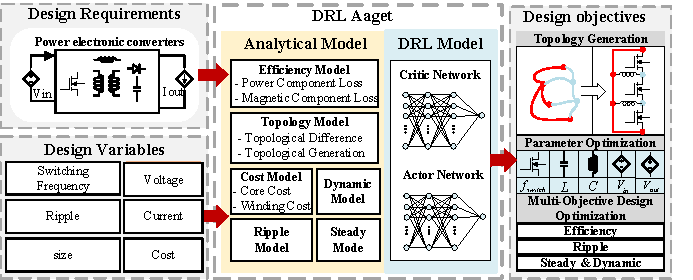
\includegraphics[width=\linewidth]{fig/design_overview2.pdf}
  \caption{General workflow of DRL-assisted converter design.}
  \label{fig:topo_overview}
\end{figure}




%%%%%%%%%%%%%%%%%%%%%%%%%%%%%%%%%%%%%%%%%%%%%%%%%%%
\subsection{Topology Exploration}
\label{sec:topo_explore}
%%%%%%%%%%%%%%%%%%%%%%%%%%%%%%%%%%%%%%%%%%%%%%%%%%%

Topology exploration has evolved rapidly with the integration of reinforcement learning (RL) and graph-based generative modeling. 
Existing approaches can be broadly categorized into adjacency-matrix-based methods, graph-learning frameworks, and hybrid generative models.

Adjacency-matrix-based strategies, such as the Q-learning framework proposed by Chen \textit{et al.}~\cite{9615058}, encode circuit connections as adjacency matrices and iteratively construct converter topologies. 
The RL agent progressively adds components under reward functions enforcing electrical feasibility and voltage–second balance, achieving fully automated topology deduction without expert intervention.  

Building upon this foundation, graph-learning frameworks employ graph neural networks (GNNs) integrated with actor–critic algorithms such as PPO~\cite{liang2022learning,10012061}. 
Liang \textit{et al.}~\cite{liang2022learning} utilized a GNN–PPO agent to sequentially attach functional blocks, reducing search complexity from exponential to near-linear. 
Dong \textit{et al.}~\cite{10012061} extended this concept by embedding voltage and current constraints into the learning policy, reducing topology generation time by an order of magnitude while lowering electrical stress by over 30\%.  

Beyond these model-driven approaches, Fan \textit{et al.}~\cite{fan2021specification} developed a hybrid upper-confidence-bound-tree (UCT) RL framework that generates converter topologies directly from target specifications. 
The agent explores feasible circuit configurations using specification-encoded rewards and a default policy trained from limited datasets, achieving up to 67\% faster generation than conventional search schemes.  
More recently, Xu \textit{et al.}~\cite{xu2022power} introduced a variational autoencoder (VAE)–RL hybrid named TopoDiffVAE, 
where a constraint-aware decoder ensures electrical validity while enhancing topological diversity.  

These studies collectively demonstrate that the synergy of RL, GNNs, and generative modeling provides a scalable and automated path for converter topology synthesis. 
The incorporation of constraint embedding and domain-specific reward shaping ensures physical realizability and supports rapid design-space exploration. 
Table~\ref{tab:Topology_Exploration} summarizes representative DRL frameworks for topology discovery in PECs.


\subsection{Parameter Optimization}
\label{sec:param_opt}

Parameter optimization plays a central role in achieving high efficiency, compact design, and thermal stability in PECs. 
Traditional workflows, dominated by manual tuning and iterative simulation, are computationally demanding and often inadequate for nonlinear parameter interactions.  
DRL provides a scalable alternative, enabling adaptive and automated search over multi-dimensional design spaces while respecting key physical and operational constraints.

\textbf{(1) Magnetic and Passive Component Optimization:}  
Recent studies have employed DQN and DDPG agents to optimize inductor geometry, air-gap length, and core material under coupled electrical–thermal constraints~\cite{tian2022deep,tian2022parameter,tian2024optimizing}.  
By integrating neural-network-based loss predictors, DRL frameworks achieve rapid convergence within seconds per iteration, minimizing loss and ripple while maintaining thermal reliability.

\textbf{(2) Surrogate-Model-Assisted Optimization:}  
To alleviate simulation burdens, hybrid DRL–surrogate frameworks incorporate deep neural network (DNN) estimators to approximate efficiency or loss metrics.  
SAC and PPO agents conduct continuous parameter optimization guided by surrogate predictions, reducing computational cost by more than one order of magnitude without sacrificing accuracy~\cite{bui2022deep,bui2023deep}.  

\textbf{(3) System-Level and Multi-Physics Co-Optimization:}  
DRL has also been applied to system-level design, where electrical, thermal, and control variables interact.  
For instance, DDPG-based methods have optimized switching frequency and modulation index in high-power inverters to improve dynamic response~\cite{wang2022efficiency}.  
Thermally coupled DRL frameworks for through-silicon-via (TSV) inductors reduce thermal stress by approximately 12\% while preserving electromagnetic integrity~\cite{wang2023modeling}.  

These developments demonstrate that DRL supports hierarchical parameter optimization, spanning passive, control, and multi-physics levels.  
Table~\ref{tab:parameter_optimization_summary} summarizes representative algorithms and their performance characteristics.


\begin{table*}[!t]
\centering
\caption{Representative DRL-Based Parameter Optimization in PECs}
\label{tab:parameter_optimization_summary}
\renewcommand{\arraystretch}{1.25}
\resizebox{\textwidth}{!}{
\begin{tabular}{@{} p{2.2cm} l p{2.5cm} l p{7cm}@{}}
\toprule
\textbf{Converter Type} & \textbf{Algorithm} & \textbf{Parameters Optimized} & \textbf{Reference} & \textbf{Advantage (+) and Disadvantage (-)} \\ 
\midrule

DC-DC Buck Converter & DQN &
Winding turns; \newline
air gap; \newline
core material &
\cite{tian2022deep} &
+ Automated inductor design \newline
+ Improved efficiency under ripple and volume constraints \newline
- Sensitive to reward shaping \newline
- Limited to discrete action settings \\ 
\midrule

DC-DC Converter & DDPG &
Semiconductor loss \newline coefficients;\newline
 magnetic geometry &
\cite{tian2022parameter} &
+ Hybrid ANN-DDPG optimization \newline
+ Fast convergence with near-optimal efficiency \newline
- Requires hyperparameter tuning \newline
- Offline training dependency \\ 
\midrule

Air-Gap Inductor \newline for DC-DC \newline Converter & DDPG &
Air-gap length; \newline 
winding turns; \newline
core material &
\cite{tian2024optimizing} &
+ Rapid geometric tuning \newline
+ Lower total loss and good generalization \newline
- Computationally demanding \newline
- Limited scalability to different topologies \\ 
\midrule

General Power \newline Converter & SAC &
Inductance;\newline
 capacitance;\newline
 switching frequency &
\cite{bui2022deep} &
+ Stable convergence via surrogate model guidance \newline
+ One-order reduction in computation cost \newline
- High network complexity \newline
- Requires pre-trained surrogate \\ 
\midrule

Buck/Boost Converters & PPO &
Inductance;\newline
capacitance;\newline
 frequency &
\cite{bui2023deep} &
+ Continuous parameter tuning \newline
+ High efficiency (97.5\%/97.7\%) with reduced runtime \newline
- Sensitive to clipping ratio \newline
- Needs extensive reward calibration \\ 
\midrule

3L-ANPC Inverter & DDPG &
Switching frequency;\newline
modulation index &
\cite{wang2022efficiency} &
+ Enhanced efficiency and dynamic response \newline
+ Effective for high-power operation \newline
- Complex reward design \newline
- Requires multiple simulation episodes \\ 
\midrule

TSV On-Chip DC-DC Converter & DDPG &
Inductor geometry; \newline
thermal stress; \newline
parasitic capacitance &
\cite{wang2023modeling} &
+ Thermal-electromagnetic co-optimization \newline
+ 11.91\% reduction in thermal stress \newline
- High modeling complexity \newline
- Long training time \\ 
\bottomrule
\end{tabular}}
\end{table*}


\subsection{Multi-Objective Design Optimization}
\label{sec:multi-objective-optimization}

Converter design typically requires balancing competing objectives such as efficiency, power density, and cost.  
Compared with conventional Pareto-based methods, DRL captures nonlinear trade-offs through adaptive reward shaping and continuous policy refinement, achieving balanced solutions with reduced computational overhead.

\textbf{(1) Efficiency–Power Density Trade-Offs:}  
In resonant and multi-level converters, DDPG agents have been used to jointly optimize component sizing, switching frequency, and power density~\cite{wang2023efficiency,wang2024case}.  
Reported prototypes achieved 96.6\% efficiency and power densities above 31~kW/dm$^3$, validating the capability of DRL for efficiency–density coordination.

\textbf{(2) Constraint-Aware and Surrogate-Enhanced Optimization:}  
Hybrid SAC–DNN frameworks extend DRL to multi-objective contexts, optimizing efficiency, cost, and reliability simultaneously~\cite{bui2022deep}.  
Constraint-aware DQN variants incorporate ripple, volume, and thermal boundaries directly into the reward structure, ensuring feasibility without explicit Pareto-front computation~\cite{tian2022deep}.  

Overall, DRL enables holistic coordination across multi-objective design tasks, bridging physical constraints and computational efficiency.  
Table~\ref{tab:multi_objective_optimization} summarizes representative multi-objective DRL implementations in PECs.

\begin{table*}[t]
\centering
\caption{Representative DRL-Based Multiobjective Optimization in PECs}
\label{tab:multi_objective_optimization}
\renewcommand{\arraystretch}{1.25}
\resizebox{\textwidth}{!}{
\begin{tabular}{@{}p{1.5cm} l p{2.8cm} l p{7.2cm}@{}}
\toprule
\textbf{Converter Type} & \textbf{Algorithm} & \textbf{Optimization Objectives} & \textbf{Reference} & \textbf{Advantage (+) and Disadvantage (-)} \\ 
\midrule

LLC Resonant Converter & DDPG &
Efficiency;\newline
Power density; \newline
Volume &
\cite{wang2023efficiency} &
+ Automated efficiency-density trade-off \newline
+ Achieved 96.57\% efficiency and 31~kW/dm$^3$ power density \newline
- Limited generalization to other converter types \newline
- Requires extensive experimental calibration \\ 
\midrule

3L-ANPC Inverter & DDPG &
Efficiency; \newline
Component volume; \newline
Current ripple &
\cite{wang2024case} &
+ Improved efficiency and ripple suppression \newline
+ Compact hybrid DRL-heuristic design \newline
- Sensitive to initialization \newline
- Complex reward structure \\ 
\midrule

Multiple Converter Topologies & SAC + DNN &
Efficiency; \newline
Component sizing; \newline
Cost &
\cite{bui2022deep} &
+ Balanced multiobjective performance across ten topologies \newline
+ Stable exploration under parameter uncertainty \newline
- Requires pre-trained surrogate model \newline
- Computationally expensive \\ 
\midrule

DC-DC Converter & DQN &
Efficiency; \newline
Ripple; \newline
Volume constraints &
\cite{tian2022deep} &
+ Handles multiobjective constraints effectively \newline
+ Ensures simultaneous satisfaction of physical limits \newline
- Reward-sensitive under conflicting objectives \newline
- Convergence dependent on discrete state design \\ 
\midrule

Grid-Connected Converter & DRL-Assisted &
Stability; \newline
Dynamic response; \newline
Grid-strength; \newline adaptability &
\cite{jiang2023stability} &
+ Enhanced stability under varying grid conditions \newline
+ Validated on real-time HIL platform \newline
- High computational overhead \newline
- Limited scalability to large-scale systems \\ 
\midrule

3L-NPC-DAB Converter & DDPG &
Power loss; \newline
Multi-DoF; \newline phase-shift control; \newline
Efficiency &
\cite{feng2025deep} &
+ Coordinated multi-DoF optimization \newline
+ High-dimensional objective learning validated experimentally \newline
- Long training time \newline
- Sensitive to reward scaling \\ 
\midrule

LLC Converter & RL &
Efficiency across \newline operating points; \newline
Frequency tuning &
\cite{kruse2022parameter} &
+ Over 90\% efficiency achieved within 50 iterations \newline
+ Adaptable across operating modes \newline
- Lacks generalization to nonlinear load conditions \newline
- Dependent on fine-tuned learning rate \\ 
\bottomrule
\end{tabular}}
\end{table*}

\subsection{Emerging Trends and Outlook}
\label{sec:drl_design_trends}

Recent developments indicate that DRL is evolving from a purely data-driven optimizer to a knowledge-guided component in hybrid, physics-aware design ecosystems.  

\textbf{1) Physics-Informed and Constraint-Embedded Learning:}  
Physical constraints such as thermal limits and stability margins are increasingly embedded into reward structures, improving convergence and ensuring design feasibility.  

\textbf{2) Hybridization with Surrogate and Evolutionary Methods:}  
Integrating DRL with surrogate modeling or heuristic search accelerates convergence and mitigates sparse-reward issues, supporting near-real-time optimization.  

\textbf{3) Hierarchical and Modular Architectures:}  
Hierarchical DRL divides complex design tasks into global and local agents, enhancing scalability and interpretability.  

\textbf{4) Transfer and Continual Learning:}  
Agents trained on one topology are being reused across similar converter architectures through transfer or continual learning, significantly reducing training cost.  

Collectively, these trends signify a shift toward unified, physics-informed DRL frameworks that integrate domain knowledge with adaptive optimization.  
They form a conceptual bridge to Section~\ref{sec_control}, where similar learning principles are extended from offline design optimization to real-time converter control.


